\documentclass{article}
\usepackage[utf8]{inputenc}
\usepackage[margin=1in,left=1.5in,includefoot]{geometry}
\usepackage{booktabs}
\usepackage{graphicx}
\usepackage{hyperref}
\usepackage{wrapfig}
\usepackage{float}
\usepackage{amsmath}
\usepackage{amssymb}
\usepackage[galician]{babel}
\usepackage[most]{tcolorbox}
\usepackage{listings}
\usepackage{lmodern}
\usepackage{xcolor}
\usepackage{caption}


\newtcolorbox{clibox}{
  colback=gray!10,    % light gray background
  colframe=gray!50,   % gray border
  boxrule=0.5pt,      % border thickness
  arc=2pt,            % rounded corners
  left=6pt,
  right=6pt,
  top=6pt,
  bottom=6pt,
  fontupper=\ttfamily % monospaced font
}


% Header & Footer Stuff

\usepackage{fancyhdr}
\pagestyle{fancy}
\lhead{\emph{Visión por Computador Aplicada}}
\rhead{614G030332425}
% \fancyfoot{}
% \lfoot{Pablo Chantada Saborido \& José Romero Conde}
% \fancyfoot[R]{}

% The Main Document
\begin{document}
	\begin{center}
		\LARGE\bfseries PRÁCTICA II\\
		\small Pablo Chantada Saborido \& José Romero Conde
		\line(1,0)A{430}
	\end{center}
	
\vspace*{300pt}
	
\begin{figure}[H]
	\centering
	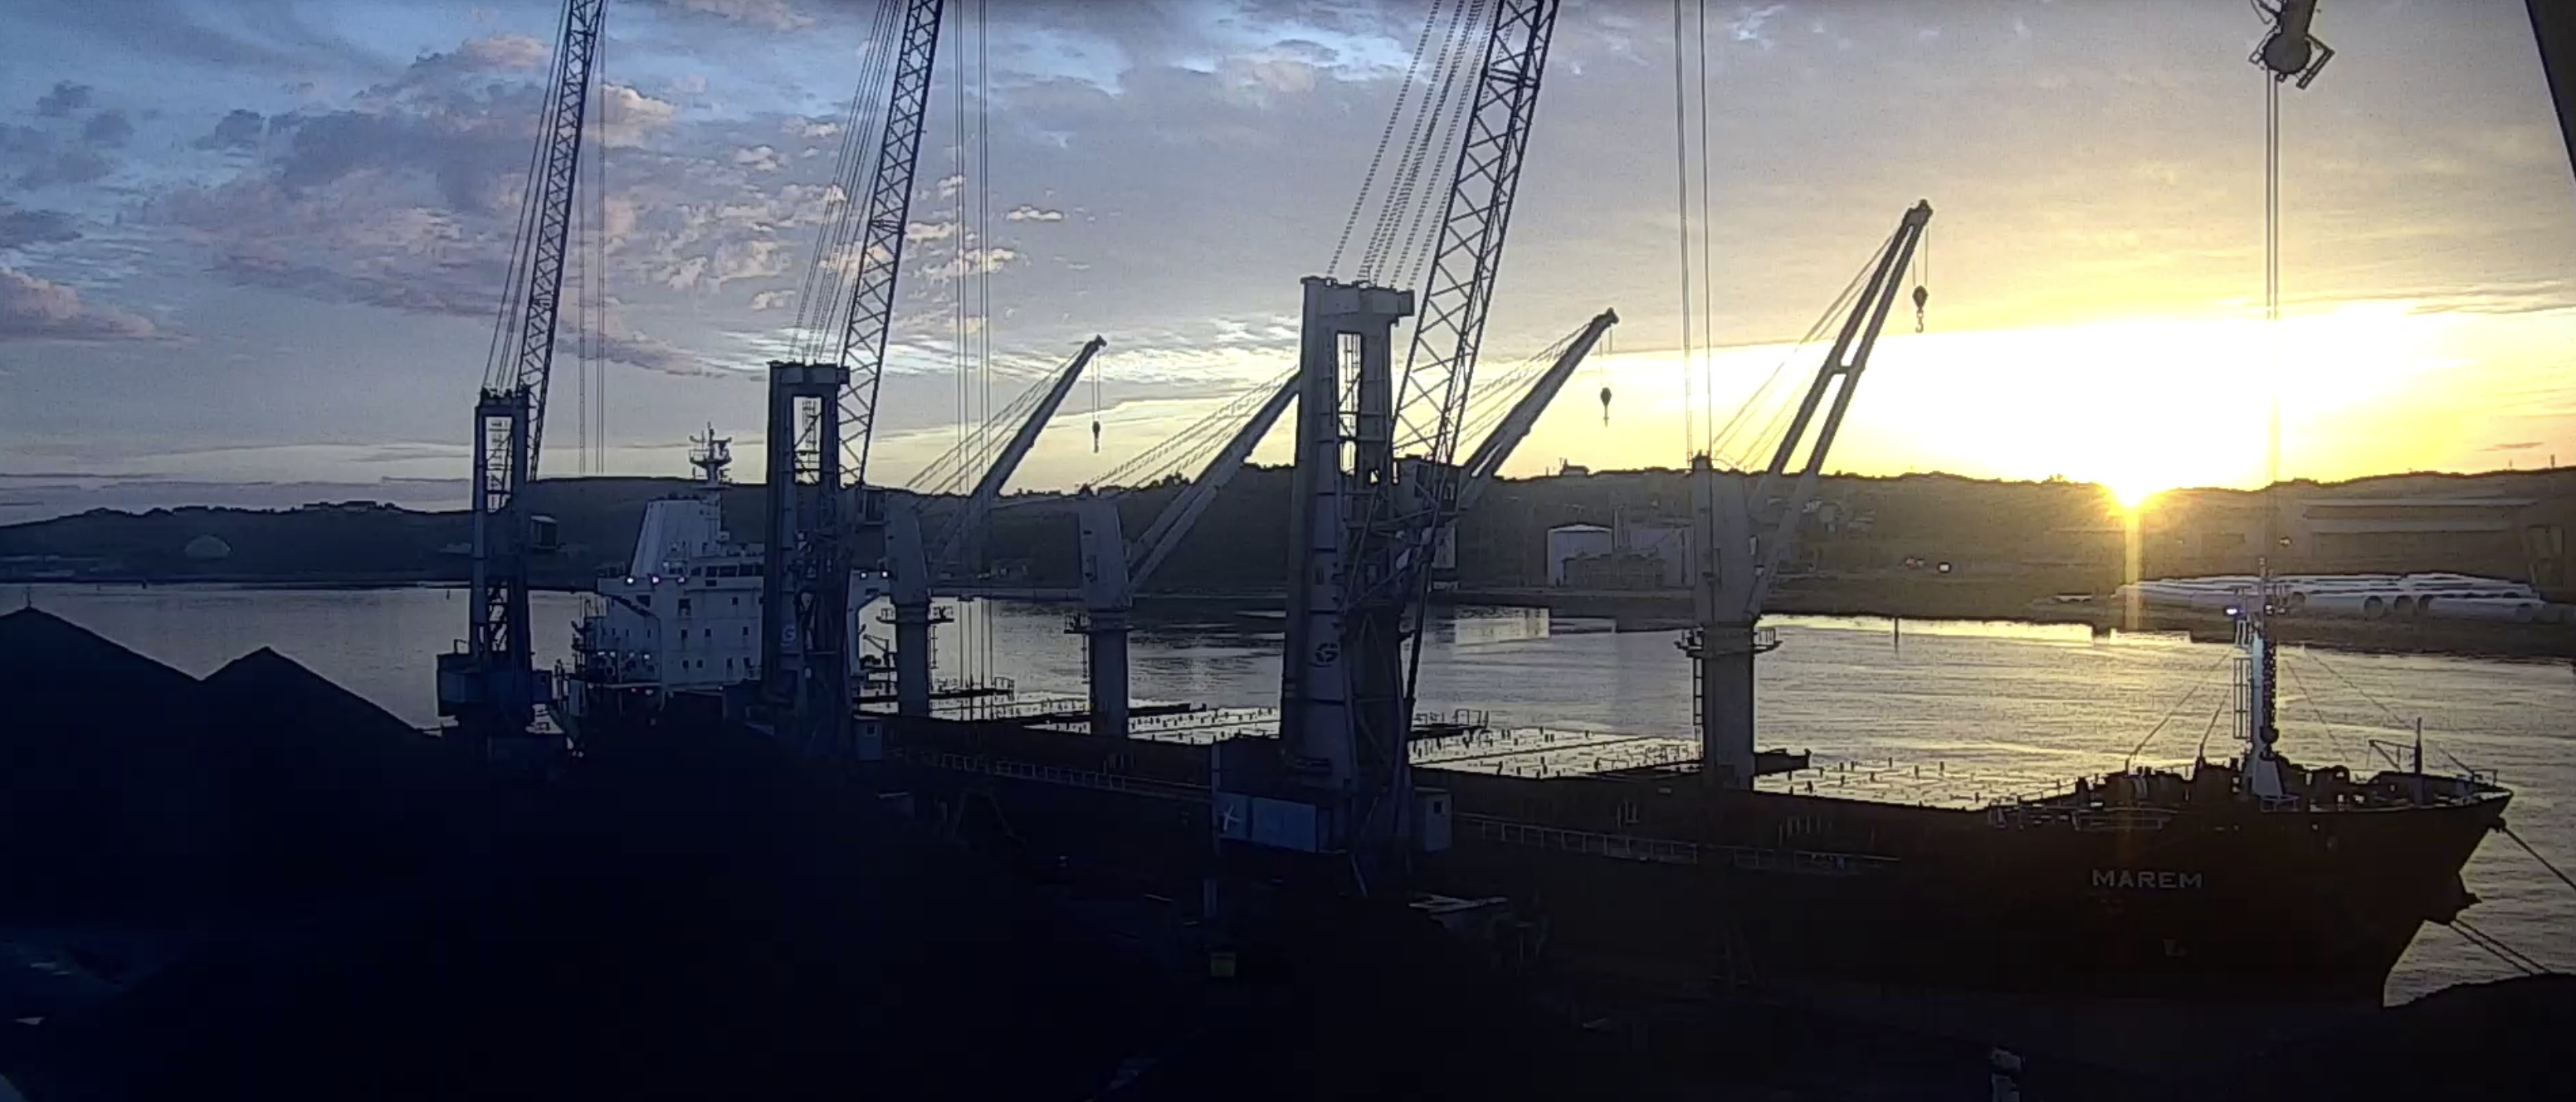
\includegraphics[width=0.7\linewidth]{figuras/portada.jpg}
	\label{fig:portada}
\end{figure}
	
\thispagestyle{empty}
	
\newpage

\tableofcontents

\newpage
	
	
\section{Introdución}

Esta práctica supuso todo un reto para nos. O Conxunto de datos foi especialmente difícil polos seguintes motivos:
\begin{itemize}
	\item \textbf{Escaseza de datos.} Acostumados a miles (MNIST) ou centos (SmartPorts) de imaxes, contar con só decenas delas supuxo unha dificultade no problema a resolver. Isto débese a que a nosa Rede ten que aprender moito de cada imaxe, e saber extrapolar o aprendido a imaxes que nunca viu. Nada sixelo.
	\item \textbf{Alta variabilidade.} Se foran poucos datos pero a realidade fosse sempre moi parecida, non habería tanto problema, a cuesstión é que de unha imaxe a outra pode haber pouco que teñan en común. As hai que a parede ocular é fina e ten unha fendidura, as hai sen fendidura mais con un gran vaso, as hai sen fendidura e con múltiples vasos... esto é para nos un problema porque o fluxo óptico \emph{existe} dun xeito distinto en cada imaxe de OCT. Polo tanto a nosa Rede debe aprender todas esas variacións con poucos exemplos.
	\item \textbf{Imperfectude da supervision.} Aínda que poderíamos ter feito un AutoEncoder para cercionarnos de unha boa representación \emph{latente}, limitámonos ó uso das máscaras para propagar a sinal de error. Ó non seren perfectas e consistentes as etiquetas (zoas dun certo nivel de gris rodeadas dun capilar, en unhas máscaras representábase o capilar e noutras non), non podemos esperar que o noso algoritmo o sexa. Ademáis, está baseándose exclusivamente en exemplos mentras que un médico razona e delibera en base os seus coñecementos teóricos e de domino. A nosa Rede non pode facer tal cousa.


\begin{figure}[H]
	\centering
	\includegraphics[width=\linewidth]{figuras/defecto_medico.png}
	\label{fig:defecto_medico}
\end{figure}

Arriba pode verse un exemplo que nos chamou a atención. Na area rodeada cun circulo violeta, na imaxe orixinal pódese ver tres \emph{paredes}, en cambio o GT só respetou á da dereita de todo e a do medio a suxeriu pero non a remetou e a da esquerda, o GT nin a asomou. En cambio a nosa Rede, sí tivo en conta a primeira parede. Este exemplo mostra que o GT non é perfecto e que, perseguilo pode ofrecer bos resultados pero só ate un punto. Por outro lado, no hospital cando fora a usarse a Rede, igoal non importa se segmenta ben esa parede, nos non podemos sabelo pero una revisión dun blog médico \cite{paxinaOCT} suxire que probablemente ese nivel de detalle non sexa importante.

\end{itemize}

Para afrotalo problema, por tanto, armamosnos con unha serie de técnicas e trucos aprendidos nesta asignatura, en Aprendizaxe Profundo e mais en Principios de Visión por Computador. Son os seguintes:
\begin{itemize}
	\item \textbf{Canles adicionais de entrada.} A Rede ten que aprender que é o fluxo óptico dende cero, sen saber que é un borde ou un círculo. Non lle pasa o mesmo ós médicos, que cando empezan na oftalmoloxía xa teñen un adestrado sistema de percepción visual. Polo tanto, para axilizar este proceso, ademáis da imaxe en Blanco e Negro $\mathcal{I}$ (un canle) decidimos acompañala dos $\phi_i(\mathcal{I})$ onde os $\phi_i$ son algoritmos de procesado de imaxen. Inicialmente escollemos Canny \cite{canny1986computational}, Sobel, Laplaciano e Frangi \cite{frangi1998multiscale}. Do último tiñamos altas esperanzas por estar tamén orientado ó ambito médico máis aínda despoís dunha considerable búsqueda de hiperparámetros decidimos descartalo para, finalmente, só quedarnos con Canny. Unha xustificación desta decisión é a imaxe de abaixo. 

\begin{figure}[H]
	\centering
	\includegraphics[width=\linewidth]{figuras/canles.png}
	\label{fig:canles}
\end{figure}


\item \textbf{Aumento de datos.} Fundamentalmente baseámonos nas suxerencias do propio artigo da UNet \cite{ronneberger2015u}  é dicir: transformacións afíns e elásticas. Cas primeiras foi realtivamente doado atopar hiperparámetros apropiados pero as segundas foi máis difícil, en cambio (ó estaren diseñadas para un contexto de segmentación médica) ofreceron moi bos resultados. Finalmente atopamos $\alpha = 500$ e $\sigma = 20$ axeitados. Ademáis, para estas dúas transformacións, ó seren realativamente \emph{agresivas}, atopamos que é millor non transformar sempre (para darlle á Rede uns poucos exemplos inalterados e aprenda deles). En concreto aplicamos cada unha delas cunha probabilidade de 0.7, polo tanto, para unha imaxen, a probabilidade de seren alterada por ambas transformacións é de $\approx 0.5$. Ademáis destas dous, aplicamos (malia observando pouca diferencia) volteos horizontais, deformacións na cor (\emph{color jitter}), variacións no enfoque e ruído gausiano aditivo. O efecto da totalidade das transformacións sobre un subconxunto das imaxes do conxunto de datos vése abaixo.

\begin{figure}[H]
	\centering
	\includegraphics[width=\linewidth]{figuras/aumento_datos.png}
	\label{fig:AD}
\end{figure}


Se ben pode parecer \emph{leve}, aumentos de datos máis agresivos non veían a luz da converxencia. Podemos dicir que a configuración de hiperparámetros do Aumento de Datos está fortemente baseada na experimentación. Comentar que tamén probamos a recortar as imaxes contrando a máscara como forma de aumento de datos pero encontramos que empeoraba o rendemento; ese tipo de cousas poden ser útiles para tareas de clasificación pero como a segmentación depende da escala en concreto e no Conxunto de Datos sempre era realtivamente a mesma escala, facer grandes variacións nese sentido pode (como temos visto) empeorar o rendemento da Rede.

\item \textbf{PostProcesado das máscaras.} Aínda que non-diferenciables, e por tanto non contribuían á sinal de error do adestramento do algoritmo, decidimos aplicar unha serie de transformacións sobre as máscaras para acercarse máis ás reais. Pulindo detalles de xeito que, se un oftalmólogo tivera que usar o noso sistema, certas impurezas corrixibles non o molestarían. En concreto nos axudamos do operador morfolóxico de peche.

\begin{figure}[H]
	\centering
	\includegraphics[width=\linewidth]{figuras/peche.png}
	\label{fig:peche}
\end{figure}

Comentar, non obstante, que por non ser o obxectivo da práctica o resultado final senón o adestramento da Rede en sí mesma, limitámonos a unha primeira idea de só aplicar peche, máis de seguro poderíanse implementarse máis e mellores alternativas.

\item \textbf{\emph{Trucos} no adestrado da Rede.} Para asegurar converxencia e acelerar o adestramento usamos Dropout \cite{srivastava2014dropout} como regularización e AdamW \cite{loshchilov2019decoupled} como optimizador que tamén implementa regularización a través dos pesos. Estos dous elementos permitiron que se propagase axeitadamente a sinal de error na Rede, que nalgúns experimentos fixemos moi grande. Adicionalmente, adicando un subconxunto dos datos a \emph{validación}, implentamos \emph{EarlyStopping} con paciencia na pérdida en validación e máis un xestor do paso de aprendizaxe que, tamén, tiña paciencia ca pérdida en valida ción. Estos dous compoñentes fixeron dinámicos parámetros que, de ser éstaticos e sempre iguais, non permitirian aprender con éxito ás Redes porque as Redes máis grandes precisan (en xeral) máis épocas, e un único paso de aprendizaxe pode estar ben pero non adoita explotar todo o potencial dunha Rede dada. Como última consideración, implentamos unha función de pérdida combinada, do seguinte xeito: \[\mathcal{L} = \alpha_{BCE} \times \mathcal{L}_{BCE} + \alpha_{FOCAL} \times \mathcal{L}_{FOCAL} + \alpha_{DICE} \times \mathcal{L}_{DICE} + \alpha_{IOU} \times \mathcal{L}_{IOU}\] onde nos fixamos $\alpha_{BCE} = 0.7$, $\alpha_{FOCAL} = 0.2$, $\alpha_{DICE} = 0.4$, $\alpha_{IOU} = 0.7$. Esos coeficientes fixáronse a partires de observar as primeiras gráficas de adestramento. Abaixo pódese ver unha grafica ca función de pérdida aquí descrita. 

\begin{figure}[H]
	\centering
	\includegraphics[width=\linewidth]{figuras/CU_adTrue_batch10_proc7_canles32_prof4_lr0.001_factocurva_perdida.jpg}
	\label{fig:perdida_funcion}
\end{figure}

\end{itemize}

\section{O noso planteamento}

Despois de ter feito a práctica anterior, reconocemos das vantaxes dun bo planteamento inicial, tanto no nivel conceptual e máis de \emph{visión} como no nivel técnico e máis de \emph{programación}. É por isto que dende un primeiro momento planteamos a práctica como un todo, por tanto, non fixemos primero un \emph{Baseline} e logo experimentos e melloras sobre iso; en vez, dende un primeiro momento planteamos na parte de programación a interfaz necesaria para, logo, facer experimentos e atopar que combinación ofrecen bos resultados. Comentamos agora, aspectos nos que fixemos probas e as nosas conclusións:

\begin{itemize}
	\item \textbf{Tamaño das imaxes.} As primeiras Redes que adestramos (poderíamos consideralas en parte, \emph{baselines}) empregaban imaxes relativamente pequenas (por custo compacional) e moi rectangulares (200 pixeles por 500), porque observando as imaxes vimos que tiñan un ratio moi pronunciado. Isto pódese comprobar cos seguintes comandos de UNIX (no directorio das imaxes):


\begin{tcolorbox}[colback=gray!10!white, colframe=gray!50!black, 
  boxrule=0.5pt, arc=2pt, left=4pt, right=4pt, top=2pt, bottom=2pt,
  fontupper=\ttfamily\small]
\$ identify * | awk '\{print \$3\}' | awk -F'x' '\{suma += \$1/\$2; n++\} END \{print "Razon ancho-alto media:", suma/n\}' \\
\>>Razon ancho-alto media: 2.6163
\end{tcolorbox}

Posteriormente decatámonos que para que a Rede percibira propiamente as paredes do Fluxo Óptico, estas non podían ter de ancho 2 ou 3 píxeles, entón, malia seren máis computacionalmente costosos, os modelos adestrados con imaxes máis grandes ofreceros mellores resultados. Tamén decatámonos de que malia seren as imaxes moi rectangulares, a mascara sempre estaba no centro e non pagaba a pena o borde, entón, malia saber que as imaxes eran moi rectangulares, a  nosa decisión final foi de 400 por 500. 

\item \textbf{Profundidade e canles base da UNet.} Despois da lectura ó artigo \cite{ronneberger2015u}, decatámonos que a UNet, máis que un modelo en concreto, é unha concepción que pode instanciarse no xeito que o fixeron os autores, é dicir, 3 niveles de profundidade 64 canles de saída na primeira convolución, pero que fácilmente pode mutar a outras configuracións. Abaixo probamos a adestrar a Rede ca mesma configuración variando só os canles de entrada (4 primeiras imaxes) e vemos que, (como suxeriuse xa no 2012 \cite{imagenet}) canto máis grande é a Rede mellores resultados. Tamén aprobeitamos para mostrar o efecto do Dropout \cite{srivastava2014dropout} (recomendado no artigo orixinal \cite{ronneberger2015u}), que é o único que varía nas dúas imaxes de abaixo. 

\begin{figure}[htbp]
    \centering
    \begin{minipage}{0.32\textwidth}
    \centering
        \includegraphics[width=\linewidth]{figuras/8.jpg}
        \caption*{8 canles base}
    \end{minipage}
    \hfill
    \begin{minipage}{0.32\textwidth}
    \centering
        \includegraphics[width=\linewidth]{figuras/16.jpg}
        \caption*{16 canles base}
    \end{minipage}
    \hfill
    \begin{minipage}{0.32\textwidth}
    \centering
        \includegraphics[width=\linewidth]{figuras/32.jpg}
        \caption*{32 canles base}
    \end{minipage}
    \hfill
    \begin{minipage}{0.48\textwidth}
    \centering
        \includegraphics[width=\linewidth]{figuras/64.jpg}
	\caption*{64 canles base, DP = 0}
    \end{minipage}
    \hfill
    \begin{minipage}{0.48\textwidth}
    \centering
        \includegraphics[width=\linewidth]{figuras/64D.jpg}
	\caption*{64 canles base, DP = 0.1}
    \end{minipage}
    \label{fig:five-images}
\end{figure}


\end{itemize}


\section{Conclusións}

\newpage

\bibliographystyle{plain}
\bibliography{referencias}



\end{document}

